
\subsubsection{Flight Dynamics and Principles of Operation}

A quadcopter is an under-actuated system, meaning it must manage six degrees of freedom (6DOF) as shown in \cref{fig:body}, three translational and three rotational—using only four control inputs (the angular velocities of the rotors).

\begin{figure}
    \caption{The inertial and body frames of a quadcopter}
    \label{fig:body}
    \centering
    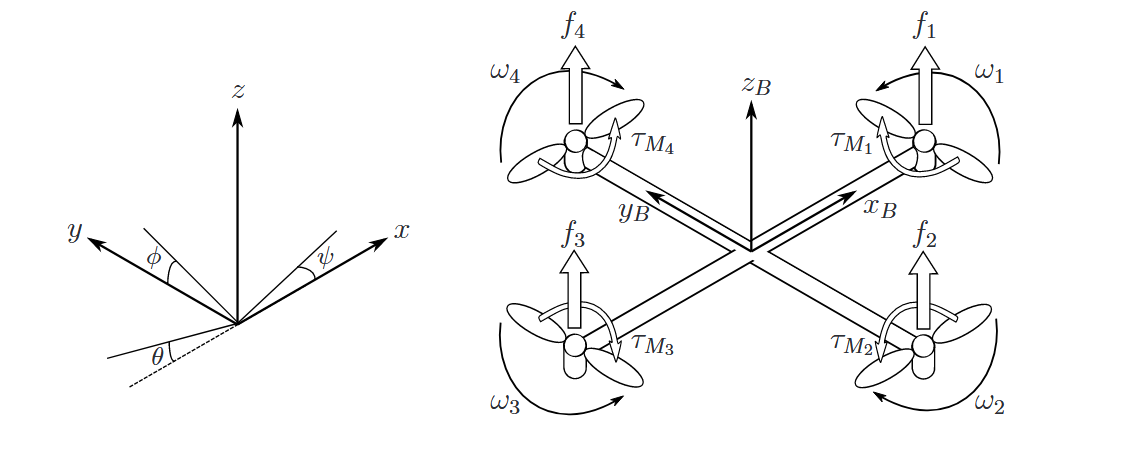
\includegraphics[width=0.8\linewidth]{img/6DOF.png}
\end{figure}

The fundamental principle of quadcopter stability relies on torque cancellation. To maintain a stable orientation, two motors rotate clockwise (CW) while the adjacent pair rotates counter-clockwise (CCW). This arrangement ensures that the net moment about the center of mass is zero; without this pair-wise opposition, the drone would rotate uncontrollably around its vertical axis. Quadcopters typically use either a "plus (+)" or "cross (x)" configuration, with the cross configuration being more common due to its superior stability \parencite{idrissi_review_2022}.


The absolute linear position of the quadcopter is defined in the inertial frame axes ($[x,y,z]^T$). The attitude, i.e. the angular position, is defined in the inertial frame with three Euler angles ($[\phi, \theta, \psi]^T$), which represent pitch angle, roll angle and yaw angle(figure 3).

Every change in position or attitude is achieved by varying the individual angular velocities ($\omega_i$) of the four rotors:

\begin{itemize}
    \item Thrust ($T$): Simultaneously increasing all rotor speeds causes the vehicle to ascend. The force generated by rotor $i$ is $f_i = k\omega_i^2$, where $k$ is the lift constant. Total thrust is defined as $T = k\sum_{i=1}^4\omega_i^2$.
    \item Yaw ($\tau_\psi$): Rotating the drone around the vertical axis is achieved by creating a torque imbalance between the CW and CCW pairs: $\tau_\psi = b (\omega_1^2 - \omega_2^2 + \omega_3^2 - \omega_4^2)$, where $b$ is the drag constant.
    \item Roll ($\tau_\phi$) and Pitch ($\tau_\theta$): These are achieved by creating a speed differential between opposite rotors. For a distance $l$ from the center of mass:
        \begin{itemize}
            \item $\tau_\phi = l k (-\omega_2^2 + \omega_4^2)$
            \item  $\tau_\theta = l k (-\omega_1^2 + \omega_3^2)$
        \end{itemize}
\end{itemize}

The quadcopter is modeled as a rigid body using Newton-Euler equations. The acceleration in the inertial frame $[x,y,z]^T$ is governed by gravity ($g$) and the orientation of the thrust vector:

$$\begin{bmatrix} \ddot{x} \\ \ddot{y} \\ \ddot{z} \end{bmatrix} = \begin{bmatrix} 0 \\ 0 \\ -g \end{bmatrix} + \frac{T}{m} \begin{bmatrix} \cos\psi \sin\theta \cos\phi + \sin\psi \sin\phi \\ \sin\psi \sin\theta \cos\phi - \cos\psi \sin\phi \\ \cos\theta \cos\phi \end{bmatrix}$$

In the body-fixed frame, the angular acceleration is influenced by the external torque ($\tau$), inertia matrix ($I$), and gyroscopic effects:

$$\begin{bmatrix} \dot{p} \\ \dot{q} \\ \dot{r} \end{bmatrix} = \begin{bmatrix} (I_{yy} - I_{zz})qr/I_{xx} \\ (I_{zz} - I_{xx})pr/I_{yy} \\ (I_{xx} - I_{yy})pq/I_{zz} \end{bmatrix} + \begin{bmatrix} \tau_\phi/I_{xx} \\ \tau_\theta/I_{yy} \\ \tau_\psi/I_{zz} \end{bmatrix}$$

